\documentclass[12pt]{article}
\usepackage[a4paper,margin=1in]{geometry}
\usepackage{xcolor}
\usepackage{tikz}
\usetikzlibrary{shapes.geometric,backgrounds}

\tikzset{
  mybackground/.style={execute at end picture={
        \begin{scope}[on background layer]
          \draw[black!15,fill=black!5] (current bounding box.south west)
                    rectangle (current bounding box.north east);
        \end{scope}
    }},
}

\setcounter{secnumdepth}{0}
\setlength{\parindent}{0pt}
\pagenumbering{gobble}

\definecolor{myBrown}{HTML}{8f754f}

\begin{document}
\begin{minipage}[t]{0.6\textwidth}
{\huge\textbf{\textcolor{myBrown}{Oskar}}} {\huge\textbf{\textcolor{myBrown}{Boer}}}\\
%+7 931 303-38-53 oskarboer@gmail.com
\section{\textcolor{myBrown}{Computer Skills}}
\section{\textcolor{myBrown}{Languages}}
\LaTeX, Pyhton, C, Bash
\section{\textcolor{myBrown}{Technologies}}
Git, Unix, SolidWorks
\section{\textcolor{myBrown}{Skills}}
3D printing, Arduino, STM32
%
\section{\textcolor{myBrown}{Education}}
\textbf{\textcolor{myBrown}{School 21}}
\begin{itemize}
\item Group work on a project
\item Prctice of clean, readable code
\item Work in enviromant with strict deadlines
\end{itemize}
\textbf{\textcolor{myBrown}{University of South Florida}}
\begin{itemize}
\item Calculus
\item SOAR engineering student comunity
\item STEM field specific english
\end{itemize}
\textbf{\textcolor{myBrown}{Physical-Technical School}}
%
\section{\textcolor{myBrown}{Interests}} 
\begin{itemize}
\item Machine learning
\item Robotics
\item Cyber security
\end{itemize}
\end{minipage}
%
\begin{minipage}{0.3\textwidth}
% \begin{tikzpicture}[mybackground={here}]
%         \node[minimum width=10in,minimum height=10in] (a) at (0,1) {};
% \end{tikzpicture}
    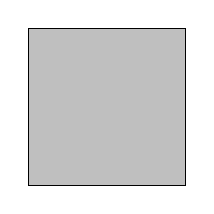
\begin{tikzpicture}
    \begin{scope}[on background layer]
        \filldraw[draw=black,fill=lightgray] (1,1) rectangle (3,3);
    \end{scope}
    \end{tikzpicture}
\end{minipage}

\end{document}